\chapter{Design}

The design phase translates the requirements identified during the system study into a structured representation of the proposed Hostel Administration System. It defines the overall architecture, functional interactions, data flow, database organisation, and user interface structure of the application. The design is intended to provide a clear separation between the different components of the system while allowing the application to be extended with additional functionality in future development.

The Hostel Administration System follows a modern full-stack web application architecture (MERN stack). The user interacts with a React-based frontend, authentication and business logic are handled through a Node.js and Express API, and application data is stored securely using MongoDB. The design also considers role-based protected access to resources so that administrative records are only accessible to authorised personnel.

\section{System Architecture}

The system architecture describes the major components of the Hostel Administration System and the manner in which they interact. The system consists primarily of the presentation layer, routing, backend API services, and document-based data storage.

The frontend is implemented using React and provides the user interfaces through which administrators and students interact with the system. React Router is used to manage navigation between different application pages. Protected routes restrict access to authenticated areas.

The backend API, built with Express.js, provides authentication and data management services. JSON Web Tokens (JWT) are used for stateless authentication. Once a user is authenticated, their role is verified by middleware to authorise operations like managing rooms or allocating students.

MongoDB provides cloud-based storage for system information. Data is organised into collections such as Users, Rooms, and Students, connected via references.

The overall architecture of the system is represented in Figure~\ref{fig:systemarchitecture}.

\begin{figure}[H]
    \centering
    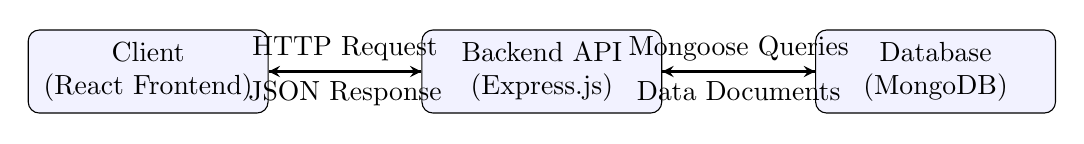
\begin{tikzpicture}[node distance=2cm, auto,
        block/.style={rectangle, draw, fill=blue!5, text width=8em, text centered, rounded corners, minimum height=3em},
        line/.style={draw, -stealth, thick}]
        
        \node [block] (client) {Client \\ (React Frontend)};
        \node [block, right of=client, node distance=5cm] (api) {Backend API \\ (Express.js)};
        \node [block, right of=api, node distance=5cm] (db) {Database \\ (MongoDB)};
        
        \path [line] (client) -- node [above] {HTTP Request} (api);
        \path [line] (api) -- node [below] {JSON Response} (client);
        
        \path [line] (api) -- node [above] {Mongoose Queries} (db);
        \path [line] (db) -- node [below] {Data Documents} (api);
    \end{tikzpicture}
    \caption{System Architecture of the Hostel Administration System}
    \label{fig:systemarchitecture}
\end{figure}

The major components of the architecture are described below.

\begin{enumerate}
    \item \textbf{Presentation Layer:} Provides the user interface using React components and Tailwind CSS.
    
    \item \textbf{Routing Layer:} Manages client-side navigation and protects authenticated routes using React Router.
    
    \item \textbf{Authentication Layer:} Provides user registration, login, logout, and token verification using Express middleware and JWT.
    
    \item \textbf{Application Service Layer:} Handles business logic operations related to room management, student allocation, and analytics.
    
    \item \textbf{Data Layer:} Uses MongoDB (via Mongoose ODM) to store and retrieve relational-like structured documents.
\end{enumerate}

\section{Use Case Design}

Use case modelling describes the functional interactions between the users and the Hostel Administration System. The primary actors of the system are the \textbf{Administrator} and the \textbf{Student}.

The major use cases identified for the system are:

\begin{itemize}
    \item Login / Logout
    \item View Dashboard
    \item Manage Rooms (Add, Edit, View)
    \item Manage Students (Register, View)
    \item Allocate Room
    \item File Complaint (Student)
\end{itemize}

The use case diagram is shown in Figure~\ref{fig:usecase}.

\begin{figure}[H]
    \centering
    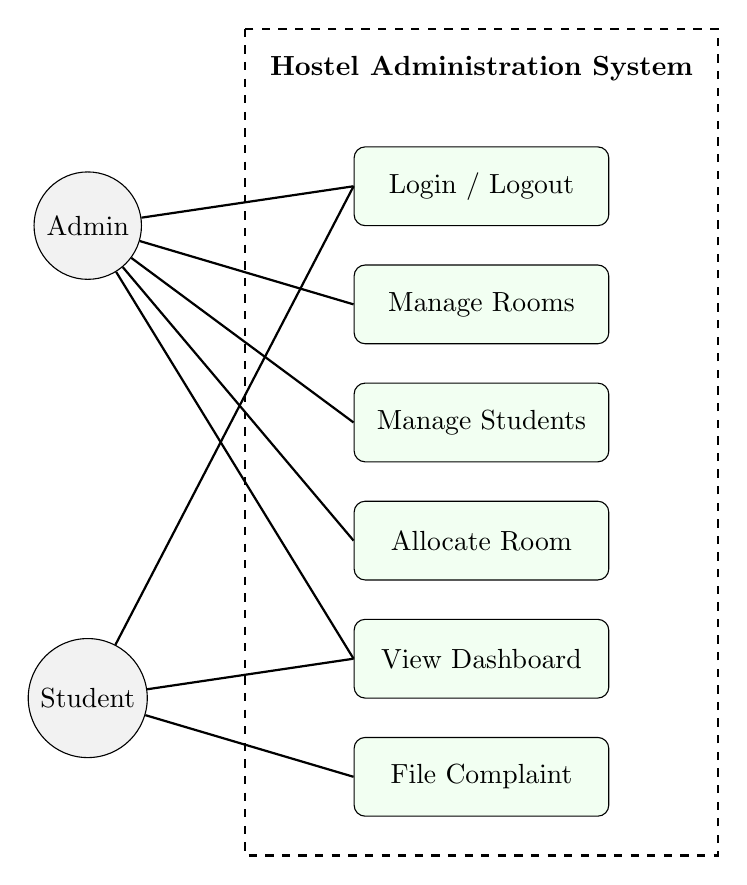
\begin{tikzpicture}[
        actor/.style={circle, draw, minimum size=1cm, fill=gray!10},
        usecase/.style={rectangle, draw, fill=green!5, rounded corners, text width=3cm, align=center, minimum height=1cm},
        line/.style={draw, thick}
    ]
        % System Boundary
        \draw[thick, dashed] (2, 2.5) rectangle (8, -8);
        \node at (5, 2) {\textbf{Hostel Administration System}};

        % Actors
        \node[actor] (admin) at (0, 0) {Admin};
        \node[actor] (student) at (0, -6) {Student};
        
        % Use Cases
        \node[usecase] (login) at (5, 0.5) {Login / Logout};
        \node[usecase] (manageRooms) at (5, -1) {Manage Rooms};
        \node[usecase] (manageStudents) at (5, -2.5) {Manage Students};
        \node[usecase] (allocate) at (5, -4) {Allocate Room};
        \node[usecase] (dashboard) at (5, -5.5) {View Dashboard};
        \node[usecase] (complaints) at (5, -7) {File Complaint};
        
        % Connections Admin
        \draw[line] (admin) -- (login.west);
        \draw[line] (admin) -- (manageRooms.west);
        \draw[line] (admin) -- (manageStudents.west);
        \draw[line] (admin) -- (allocate.west);
        \draw[line] (admin) -- (dashboard.west);
        
        % Connections Student
        \draw[line] (student) -- (login.west);
        \draw[line] (student) -- (dashboard.west);
        \draw[line] (student) -- (complaints.west);
    \end{tikzpicture}
    \caption{Use Case Diagram of the Hostel Administration System}
    \label{fig:usecase}
\end{figure}

\subsection{Login / Logout}

Allows registered users (Administrators or Students) to securely access or exit the system using their credentials. Authentication generates a JWT for session management.

\subsection{View Dashboard}

Provides the main authenticated interface displaying relevant information based on the user's role, such as overall occupancy for administrators or room details for students.

\subsection{Manage Rooms}

Allows the administrator to create, update, or view hostel room records. This includes setting the capacity, current occupancy, block name, and associated facilities.

\subsection{Manage Students and Allocate Room}

Allows administrators to register student profiles and allocate them to specific available rooms. The system automatically updates room occupancy based on these allocations.

\section{Data Flow Diagram}

A Data Flow Diagram (DFD) represents the movement of information between the user, system processes, and data storage.

\subsection{Level 0 Data Flow Diagram}

At the highest level, the system can be represented as a single process interacting with users and the database. The Level 0 DFD is shown in Figure~\ref{fig:dfdlevel0}.

\begin{figure}[H]
    \centering
    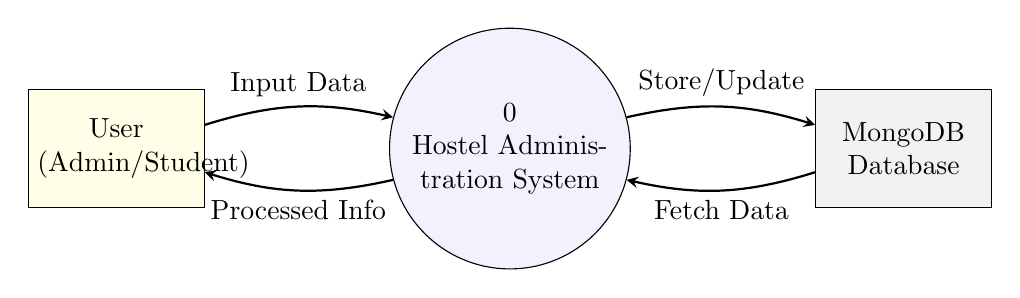
\begin{tikzpicture}[node distance=4cm, auto,
        entity/.style={rectangle, draw, fill=yellow!10, text width=2cm, text centered, minimum height=1.5cm},
        process/.style={circle, draw, fill=blue!5, text width=2.5cm, text centered, minimum height=2.5cm},
        db/.style={rectangle, draw, fill=gray!10, text width=2cm, text centered, minimum height=1.5cm},
        line/.style={draw, -stealth, thick}]
        
        \node [entity] (user) {User \\ (Admin/Student)};
        \node [process, right of=user, node distance=5cm] (system) {0 \\ Hostel Administration System};
        \node [db, right of=system, node distance=5cm] (database) {MongoDB Database};
        
        \path [line] (user) edge[bend left=15] node[above] {Input Data} (system);
        \path [line] (system) edge[bend left=15] node[below] {Processed Info} (user);
        
        \path [line] (system) edge[bend left=15] node[above] {Store/Update} (database);
        \path [line] (database) edge[bend left=15] node[below] {Fetch Data} (system);
    \end{tikzpicture}
    \caption{Level 0 Data Flow Diagram}
    \label{fig:dfdlevel0}
\end{figure}

\section{Activity Design}

Activity diagrams represent the sequence of actions involved in major operations of the system.

\subsection{User Authentication Activity}

The authentication process begins when the user enters their credentials. If valid, the backend issues a JWT, and the user is redirected to the dashboard.

\begin{figure}[H]
    \centering
    \begin{tikzpicture}[node distance=1.8cm, auto,
        start/.style={circle, draw, fill=black, minimum size=0.5cm},
        end/.style={circle, draw, fill=black, minimum size=0.5cm, double=white, double distance=1pt},
        action/.style={rectangle, draw, fill=blue!5, rounded corners, text width=3.5cm, text centered, minimum height=1cm},
        decision/.style={diamond, draw, fill=yellow!10, text width=2.5cm, text centered, inner sep=0pt},
        line/.style={draw, -stealth, thick}]
        
        \node [start] (start) {};
        \node [action, below of=start] (enter) {Enter Credentials};
        \node [action, below of=enter] (submit) {Submit to API};
        \node [decision, below of=submit, node distance=2.5cm] (check) {Credentials Valid?};
        \node [action, right of=check, node distance=4.5cm] (error) {Display Error Message};
        \node [action, below of=check, node distance=2.5cm] (auth) {Generate \& Store JWT};
        \node [action, below of=auth] (redirect) {Redirect to Dashboard};
        \node [end, below of=redirect] (end) {};
        
        \path [line] (start) -- (enter);
        \path [line] (enter) -- (submit);
        \path [line] (submit) -- (check);
        \path [line] (check) -- node [near start] {No} (error);
        \path [line] (error) |- (enter);
        \path [line] (check) -- node [near start] {Yes} (auth);
        \path [line] (auth) -- (redirect);
        \path [line] (redirect) -- (end);
    \end{tikzpicture}
    \caption{User Authentication Activity Diagram}
    \label{fig:activitylogin}
\end{figure}

\section{Database Design}

The Hostel Administration System uses MongoDB, a NoSQL document database, allowing flexible and scalable data storage. Data is organised into collections.

The database structure relies on reference relationships (ObjectIds) to associate students with specific rooms. The conceptual schema is represented below:

\begin{verbatim}
Database: HostelDB
 |
 +-- Users Collection
 |    +-- _id, name, email, passwordHash, role
 |
 +-- Rooms Collection
 |    +-- _id, roomNumber, block, capacity, occupancy, facilities
 |
 +-- Students Collection
      +-- _id, name, registrationNumber, roomId (ref: Rooms), contact
\end{verbatim}

The main fields of a Room document are described in Table~\ref{tab:roomfields}.

\begin{table}[H]
\centering
\caption{Room Document Fields}
\label{tab:roomfields}
\begin{tabular}{p{0.25\textwidth} p{0.55\textwidth}}
\toprule
\textbf{Field} & \textbf{Description} \\
\midrule
roomNumber & Unique identifier for the physical room. \\
block & The building or block where the room is located. \\
capacity & Maximum number of students the room can accommodate. \\
occupancy & Current number of students allocated to the room. \\
facilities & Array of amenities provided in the room (e.g., AC, WiFi). \\
\bottomrule
\end{tabular}
\end{table}

\section{User Interface Design}

The user interface is designed to provide a simple and accessible environment for managing hostel records. The interface follows a component-based approach using React and Tailwind CSS.

\subsection{Dashboard}

The dashboard acts as the primary interface after authentication. It provides quick statistics (e.g., total rooms, available beds) and navigation links to specific management modules.

\subsection{Add Room Form}

The Add Room form allows an administrator to define new accommodation spaces. 

\begin{figure}[H]
    \centering
    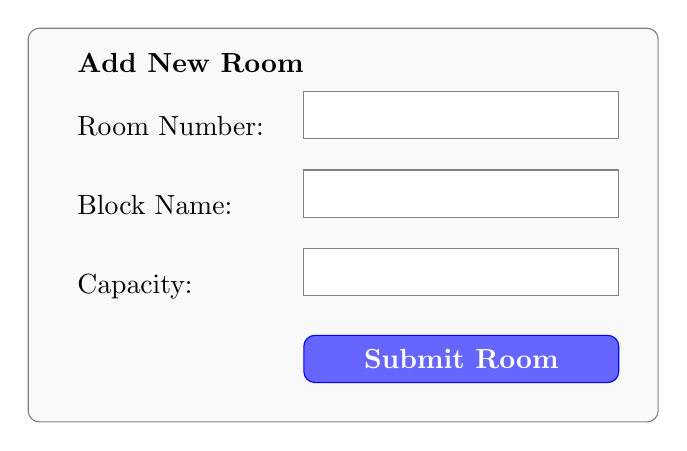
\begin{tikzpicture}
        \draw[fill=gray!5, draw=gray, rounded corners] (0,0) rectangle (8, 5);
        \node[anchor=north west, font=\bfseries] at (0.5, 4.8) {Add New Room};
        
        \node[anchor=north west] at (0.5, 4) {Room Number:};
        \draw[fill=white, draw=gray] (3.5, 3.6) rectangle (7.5, 4.2);
        
        \node[anchor=north west] at (0.5, 3) {Block Name:};
        \draw[fill=white, draw=gray] (3.5, 2.6) rectangle (7.5, 3.2);
        
        \node[anchor=north west] at (0.5, 2) {Capacity:};
        \draw[fill=white, draw=gray] (3.5, 1.6) rectangle (7.5, 2.2);
        
        \draw[fill=blue!60, draw=blue, rounded corners] (3.5, 0.5) rectangle (7.5, 1.1);
        \node[text=white, font=\bfseries] at (5.5, 0.8) {Submit Room};
    \end{tikzpicture}
    \caption{Wireframe representation of the Add Room Form}
    \label{fig:addroom}
\end{figure}

\section{Security Design}

Security is critical because the system stores personal student data and administrative records. 

Authentication is managed using JSON Web Tokens (JWT). When a user logs in, the server signs a token containing their user ID and role. This token must be included in the headers of subsequent API requests.

Protected routes in React prevent unauthenticated users from accessing administrative pages. On the backend, Express middleware intercepts requests to verify the JWT and checks the user's role before permitting database operations (e.g., only an 'admin' can delete a room record).

\section{Design Summary}

The design of the Hostel Administration System defines the architecture, functional interactions, data flow, database structure, and interface components required. The MERN stack architecture cleanly separates the user interface, routing, API services, and data storage, ensuring the system remains modular and extensible.

The use case model and DFDs identify the major interactions available to administrators and students, while TikZ diagrams provide a visual representation of system architecture and activity flows. The MongoDB document structure provides relational data tracking for room allocations, establishing a robust foundation for the implementation phase.
